
\documentclass[12pt,a4paper,oneside]{article}
\usepackage[margin=1.2in]{geometry}
\usepackage{appendix}
\usepackage[dvips]{graphicx}
\usepackage{epsfig}
\usepackage{amsmath}
\usepackage{amssymb}
\usepackage{psfrag}
\usepackage[square, comma,sort,numbers]{natbib}
\usepackage{fancyhdr}
\usepackage[nottoc]{tocbibind}
\usepackage{color}
\usepackage{fixltx2e}
\usepackage{pdfpages}
\usepackage{pdflscape}
\usepackage{booktabs}
\usepackage{graphicx}
\usepackage{float}
\usepackage{afterpage}
\usepackage{subcaption}
\usepackage{lscape}
\usepackage{rotating}
\usepackage{enumitem}
\usepackage{array,tabularx}
\usepackage{fancyref}
\usepackage[dvipsnames]{xcolor}
\usepackage[colorlinks=true,allcolors=blue]{hyperref}%



\newcommand{\quotes}[1]{``#1''}

\newenvironment{conditions*}
  {\par\vspace{\abovedisplayskip}\noindent
   \tabularx{\columnwidth}{>{$}l<{$} @{\ : } >{\raggedright\arraybackslash}X}}
  {\endtabularx\par\vspace{\belowdisplayskip}}



\pagestyle{fancy}
\title{\Huge The Hat Creek Radio Observatory\\
\vspace{0.5cm}
Screen Room Tests\\
\vspace{0.5cm}
\normalsize \emph{}
\vspace{3.5cm}
\begin{center}

\includegraphics[height=4cm]{titlepage/SETI_institute_logo.jpg}
\end{center}
}
\author{ 
\vspace{1cm}
\Large
\textbf{ Alexander Pollak \& Marc Jacquart} \\
SETI Institute \\ 
339 Bernardo Ave, Suite 200 \\
Mountain View, CA 94043 \\ 
Alexander.Pollak.87@gmail.com\\
}
\date{\today}



\begin{document}
\clearpage\maketitle
\thispagestyle{empty}

%\newpage
%\thispagestyle{empty}
%\section*{Abstract}
%\noindent 
%



%
%\vspace{3cm}
%\begin{flushright}
%Alexander Pollak \\ \emph{September, 2015}
%\end{flushright}

%\newpage
%\thispagestyle{empty}
%\tableofcontents
\newpage

%----------------------------------------------------------------------------------------
%	General
%----------------------------------------------------------------------------------------
%\pagestyle{plain}
\section{General}
\label{sec:General}
% ----------------------------------------------------------------
A screen room (figure \ref{fig:screen_room_outside}) has been built in the "Lab 2" building to test new RF equipment. A metallic mesh around the room acts as a Faraday cage and shields the ATA from electromagnetic interferences from the tests inside the room. The measurement of the shielding effectiveness are described in this document.


\begin{figure}[H]
\centering
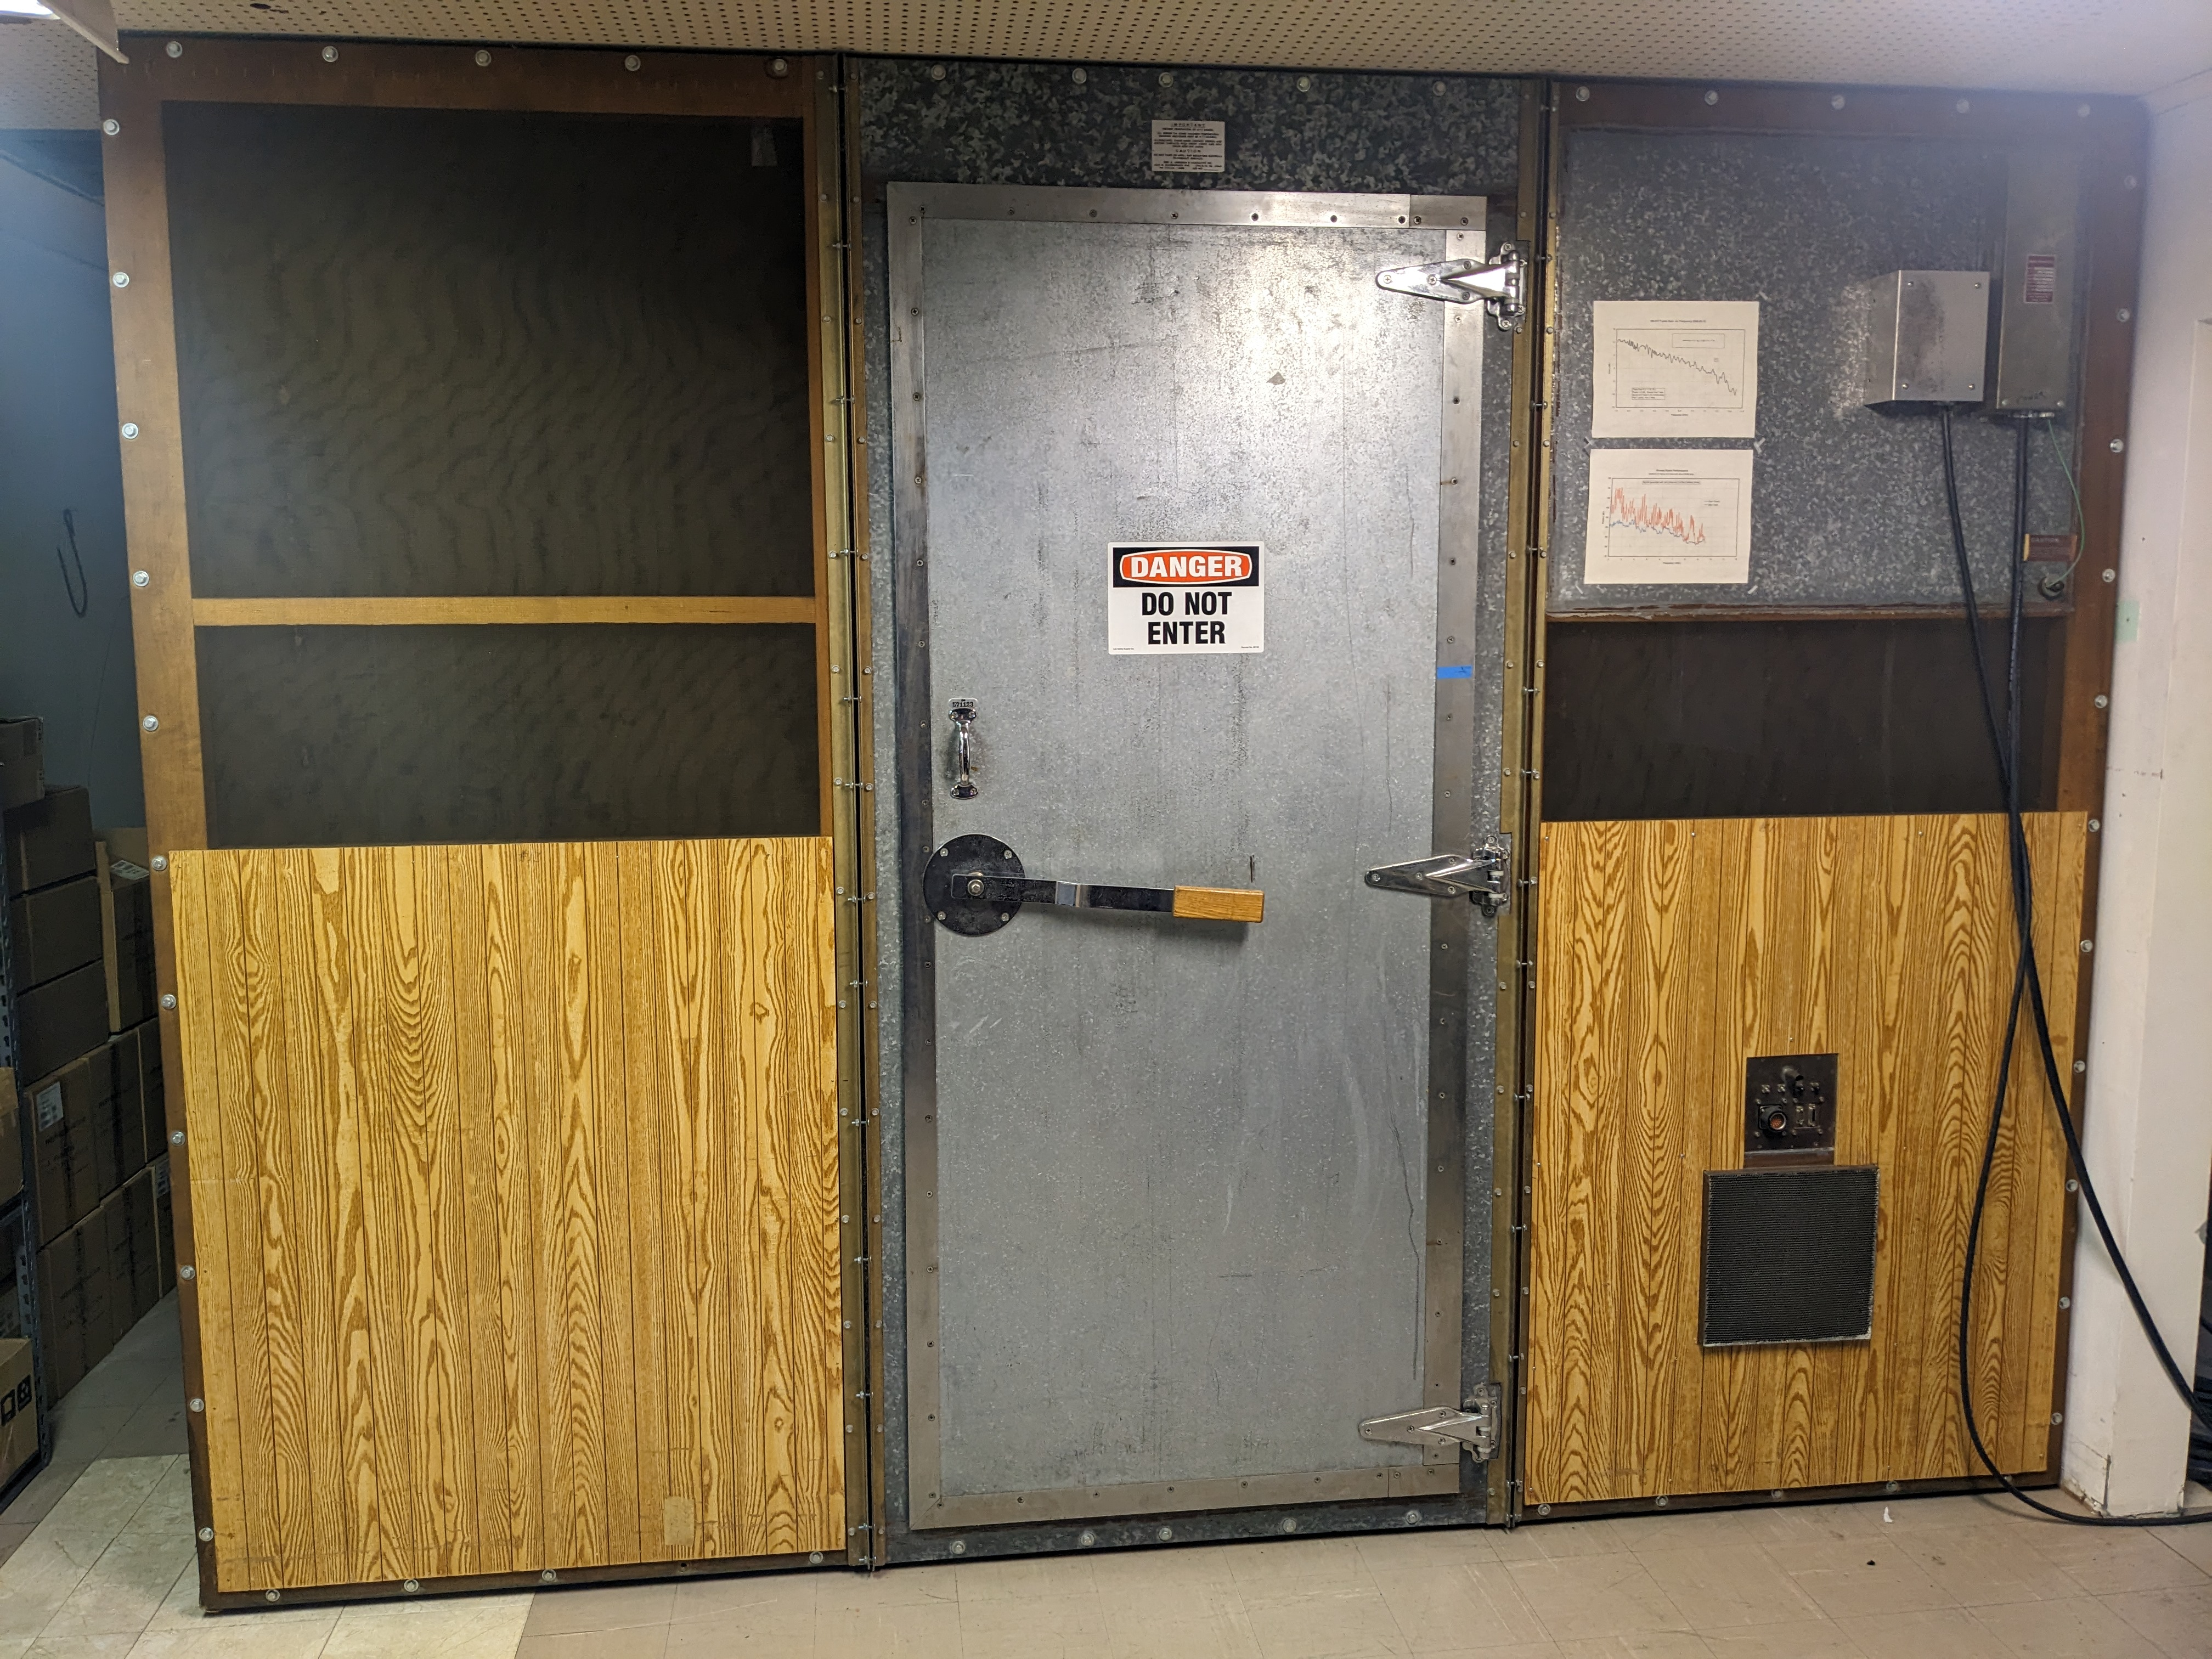
\includegraphics[width=1\linewidth]{images/screen_room.jpg}
\caption{Outside view of the screen room in the "Lab 2".}
\label{fig:screen_room_outside}
\end{figure}


\section{Testing setup}
\label{sec:Testing}
The shielding effectiveness of the screen room is tested with a radio emitter and receiver. The emitter is made from an "E4420B Agilent RF Generator" connected to an "OmniLOG 30800" omnidirectional antenna with a two-meter Female-Female SMA cable "ABC-CA18-SMSM-2.OM". The antenna is placed at the center of the room on a tripod and the RF generator emits a +20$\thinspace$dBm signal first at 800$\thinspace$MHz, then at 2$\thinspace$GHz. A schematic of the emitter setup is shown in figure \ref{fig:schematic_emitter} and a picture in figure \ref{fig:function_generator}.

The receiver is held by hand around the room to make several power level measurement around the room. The "Keysight N9938A FieldFox Microwave Spectrum Analyzer" is connected to a RF-preamplifier "Aaronia UBBV X 17823" which is then connected to an "OmniLOG 30800" omnidirectional antenna. Only the power level is recorded at the frequency we know is emitted inside the screen room. \textbf{TODO: Add more details on the measurement} A schematic of the receiver setup is shown in figure \ref{fig:schematic_receiver} and a picture in figure \ref{fig:spectrum_analyzer}.

\textbf{TODO: ADD spectrum analyzer settings list.}
\begin{figure}[H]
\centering
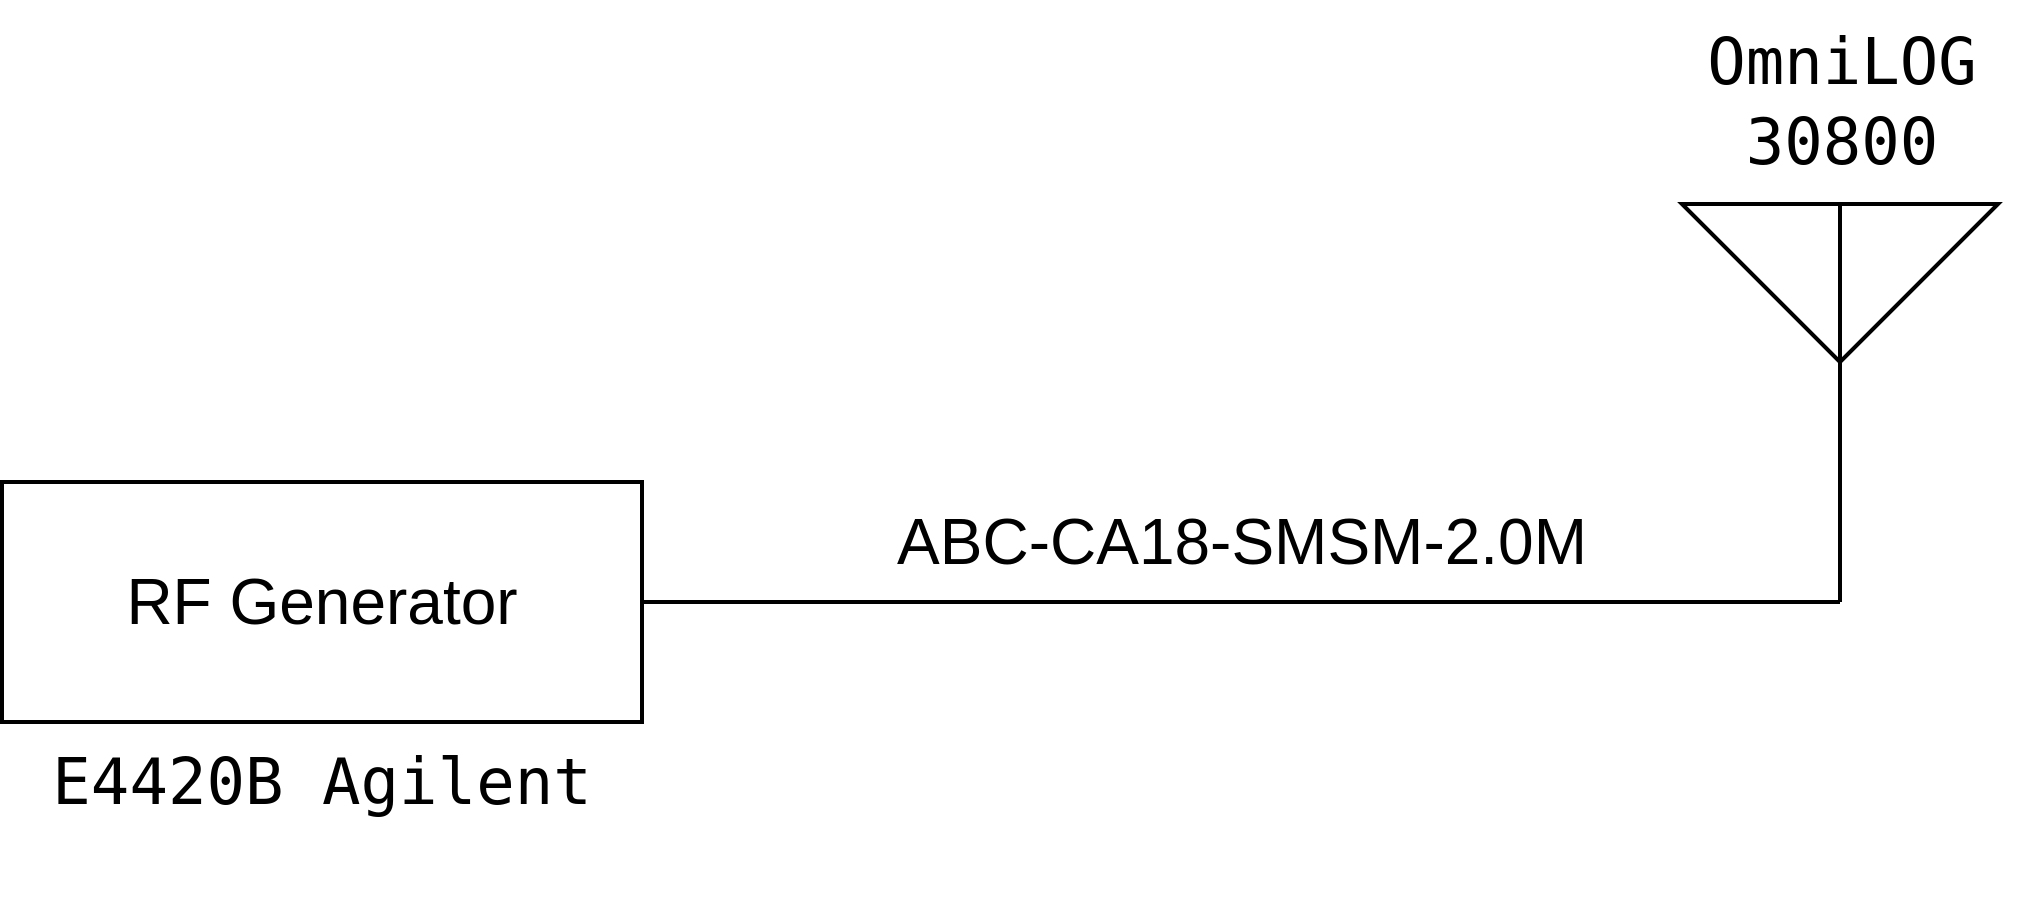
\includegraphics[width=0.8\linewidth]{images/schematics/emitter.png}
\caption{Schematic of the emitter test setup.}
\label{fig:schematic_emitter}
\end{figure}

\begin{figure}[H]
	\centering
	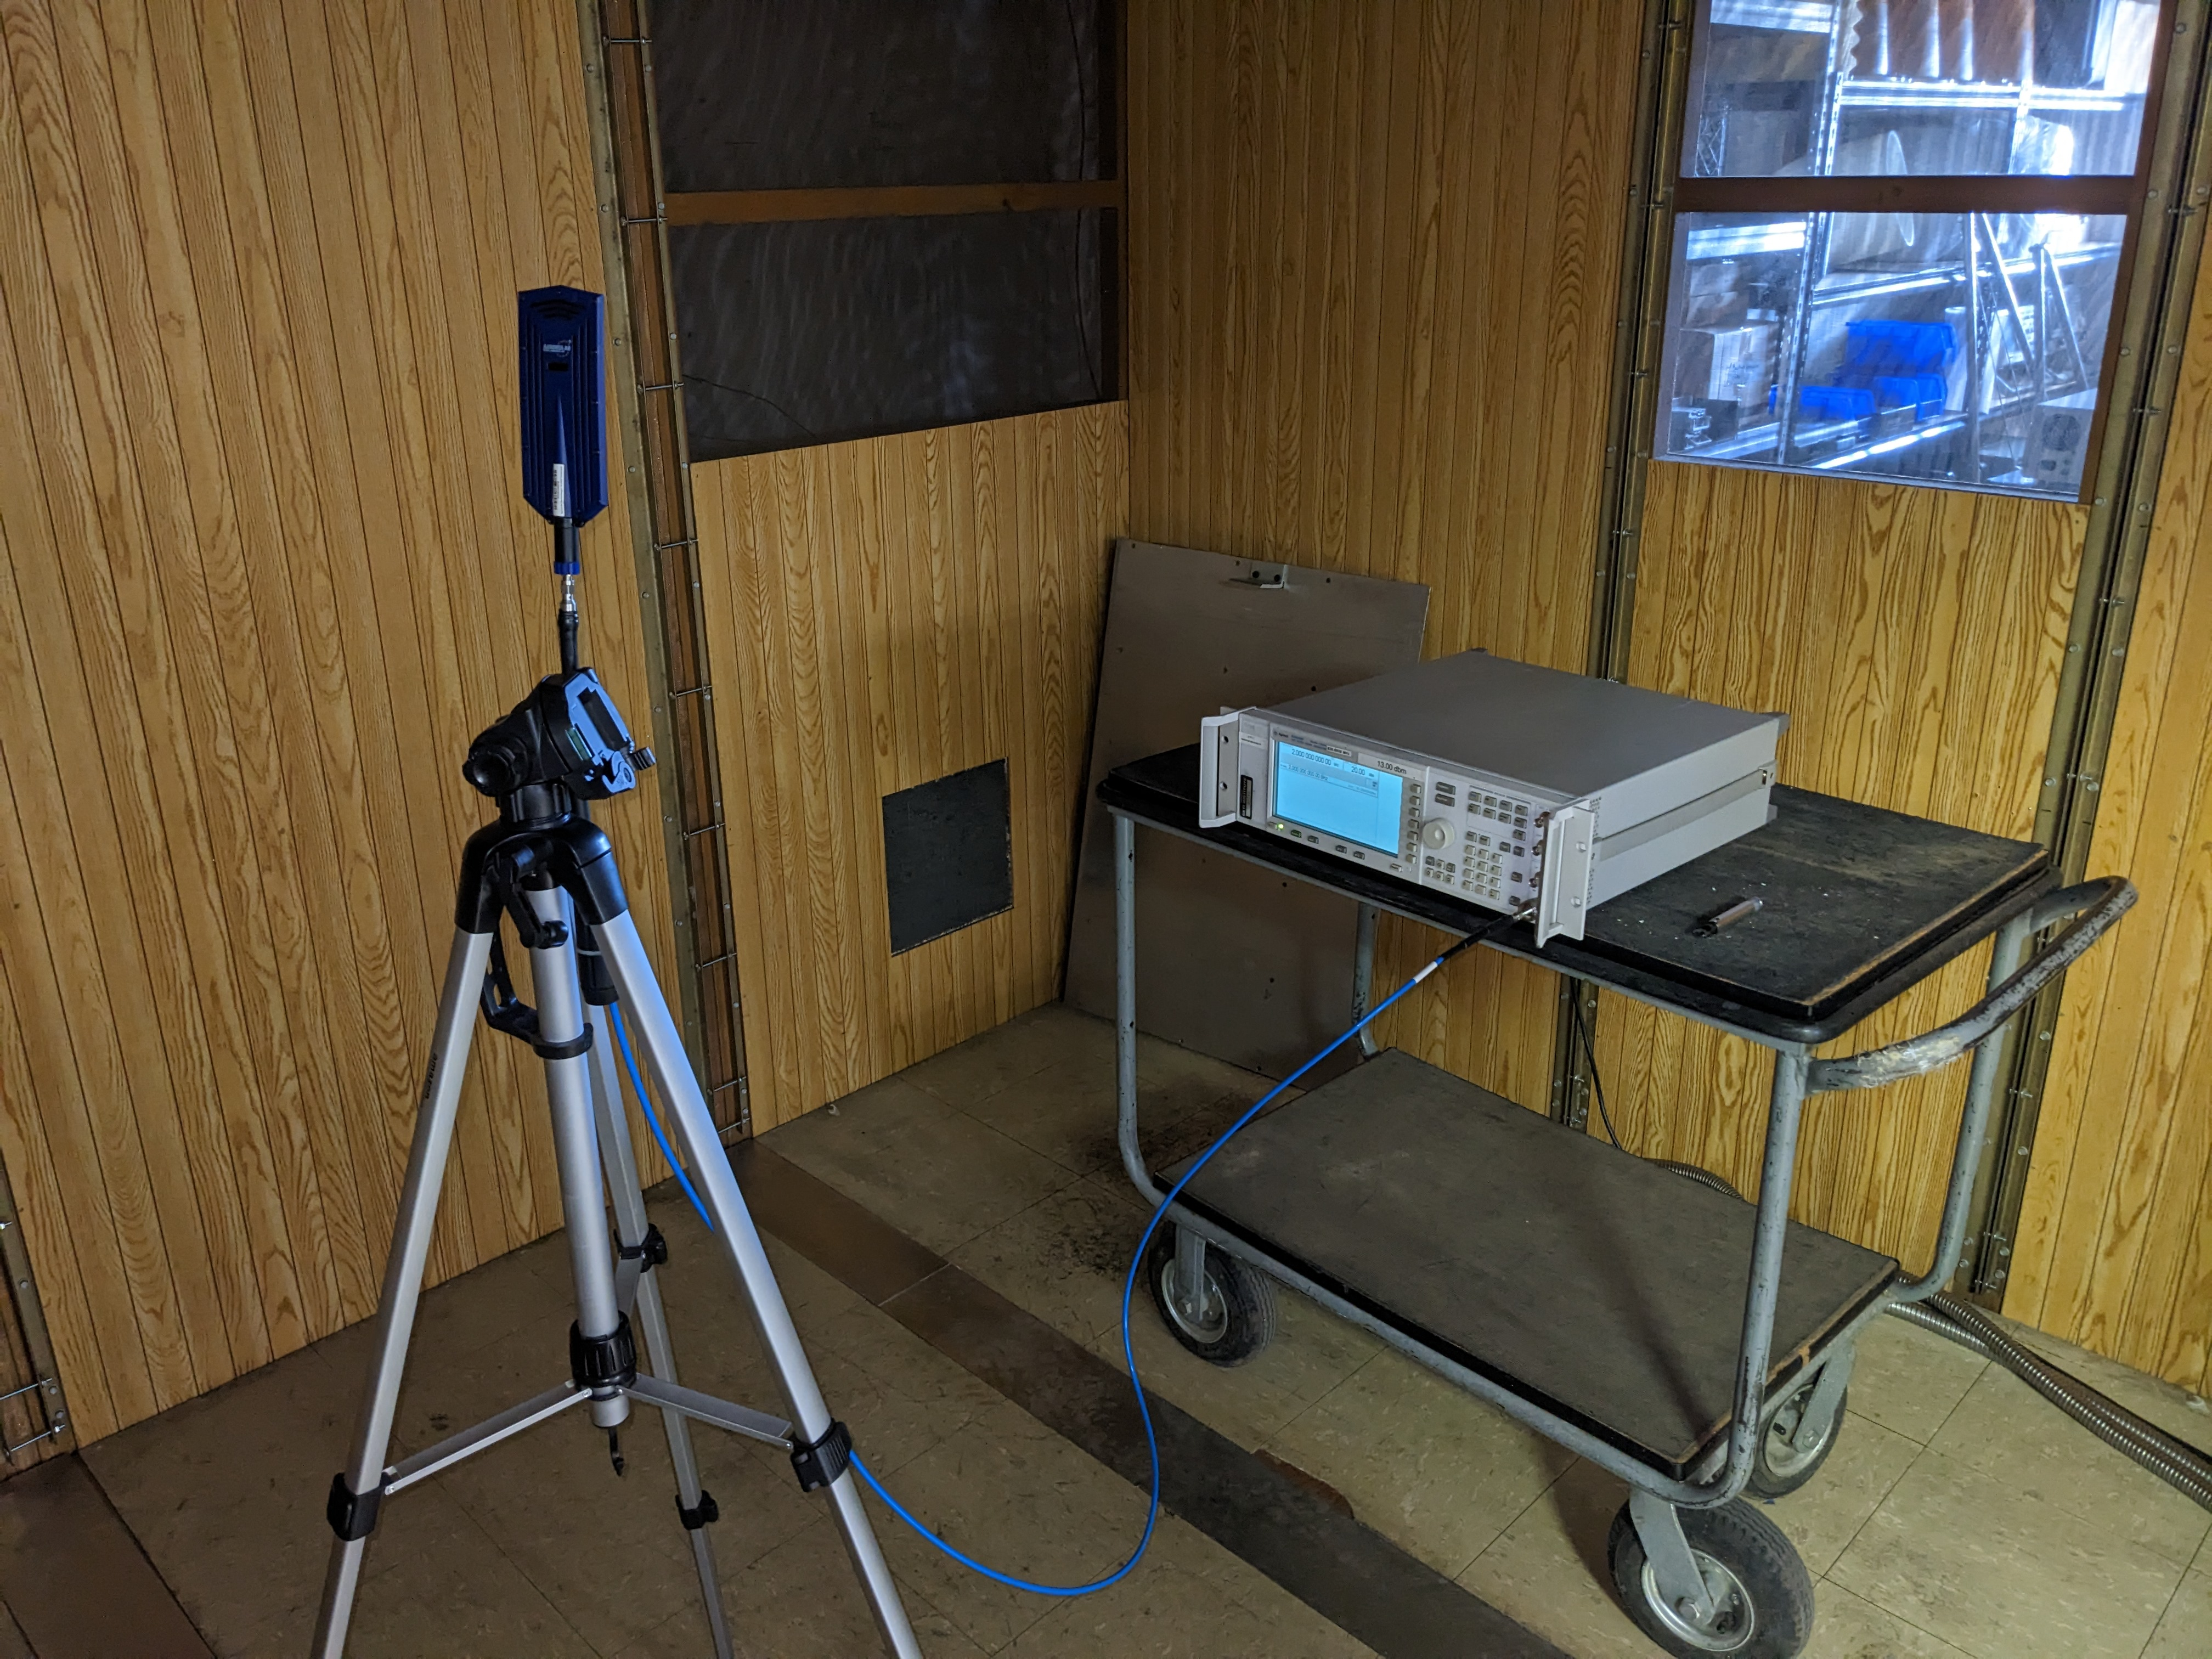
\includegraphics[width=0.9\linewidth]{images/function_generator.jpg}
	\caption{Function generator emitting through a omnidirectional antenna in the middle of the screen room.}
	\label{fig:function_generator}
\end{figure}

\begin{figure}[H]
\centering
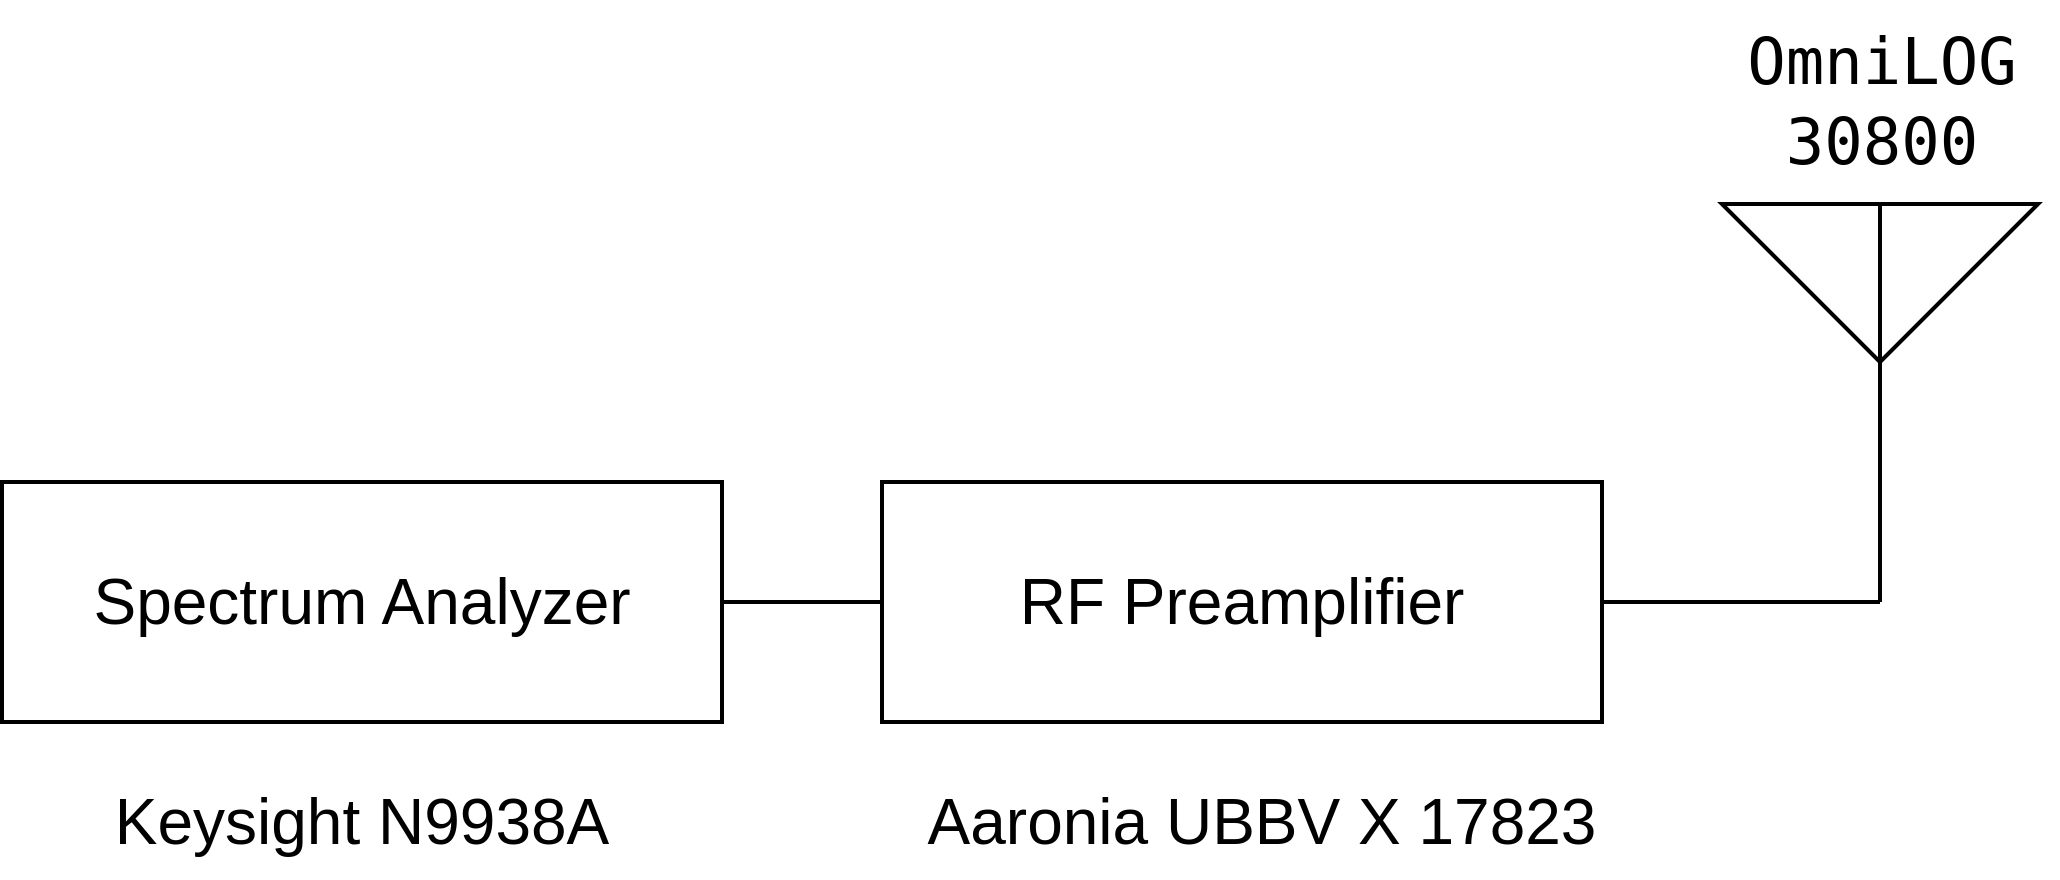
\includegraphics[width=0.8\linewidth]{images/schematics/receiver.png}
\caption{Schematic of the receiver test setup.}
\label{fig:schematic_receiver}
\end{figure}

\begin{figure}[H]
	\centering
	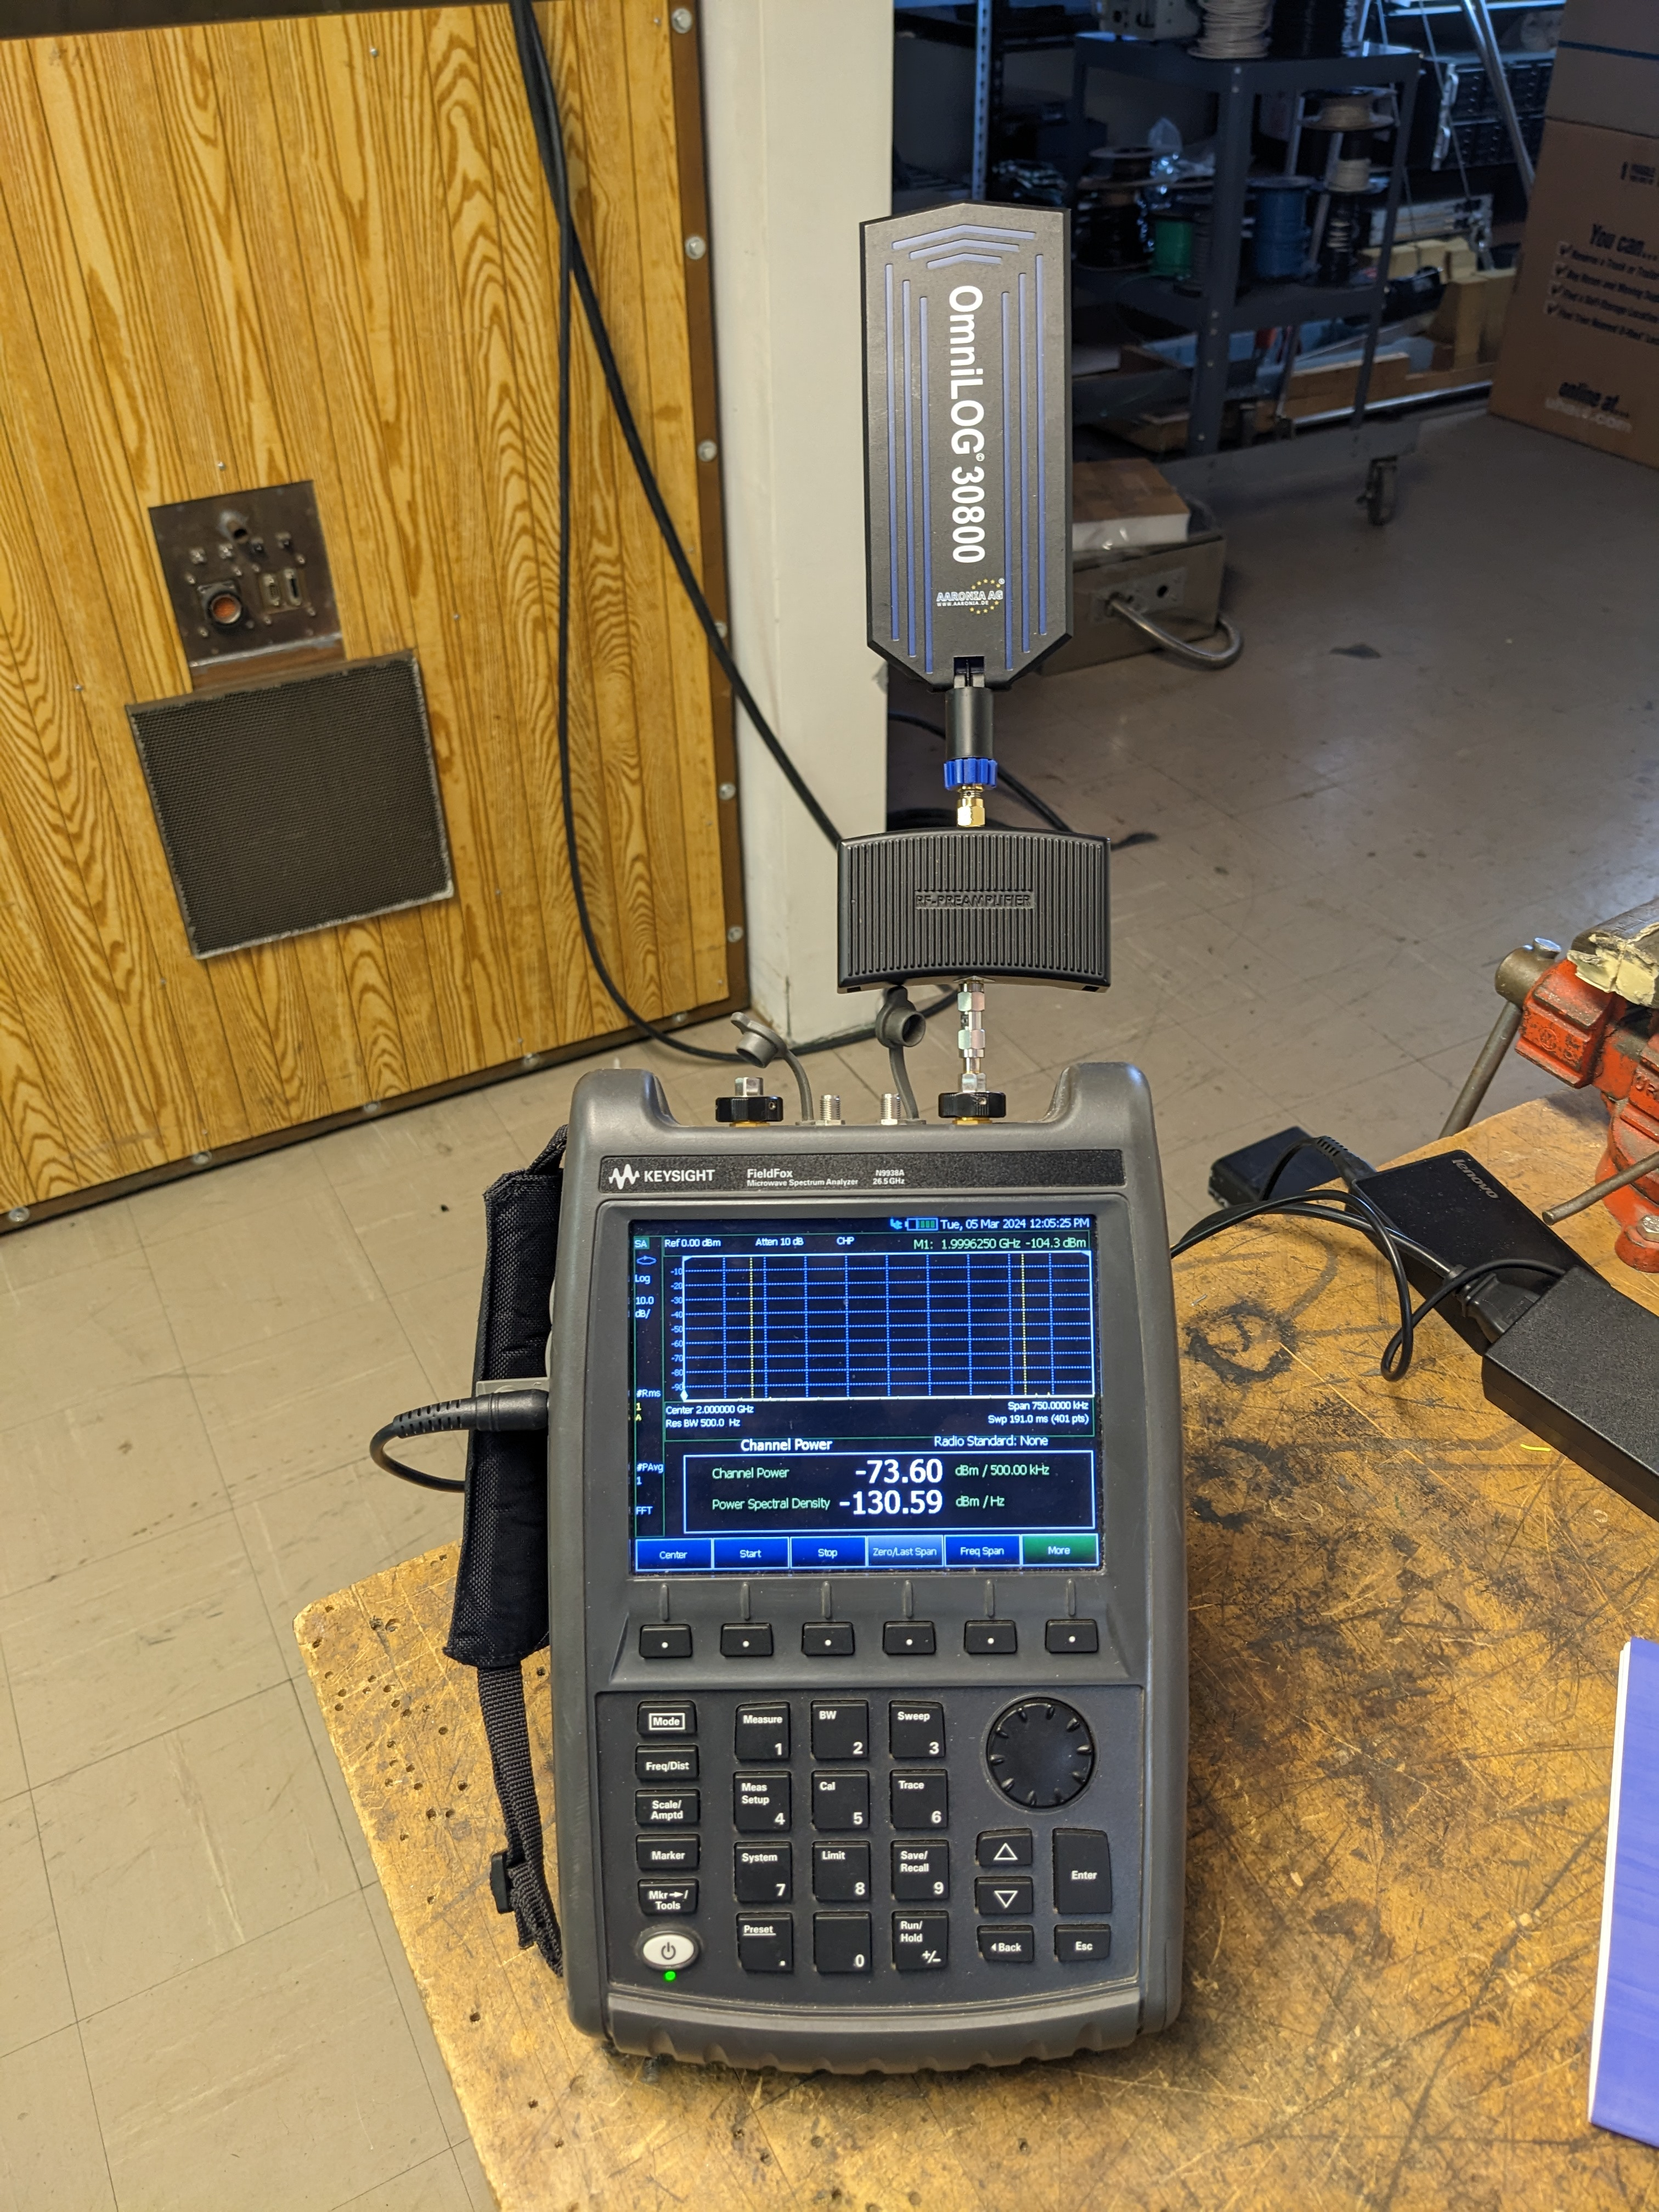
\includegraphics[width=0.75\linewidth]{images/spectrum_analyzer.jpg}
	\caption{The spectrum analyzer used for the measurement, connected to the antenna through a signal amplifier.}
	\label{fig:spectrum_analyzer}
\end{figure}

% ----------------------------------------------------------------

\subsection{Results}
\label{sec:Results}
The result of the measurements for both 800$\thinspace$MHz and 2$\thinspace$GHz are shown in in figure \ref{fig:800MHz_result} and \ref{fig:2GHz_result} respectively. The $-5\thinspace$dB measurement indicates a signal leak at the right of the door and the problem will need to be fixed.

\begin{figure}[H]
\centering
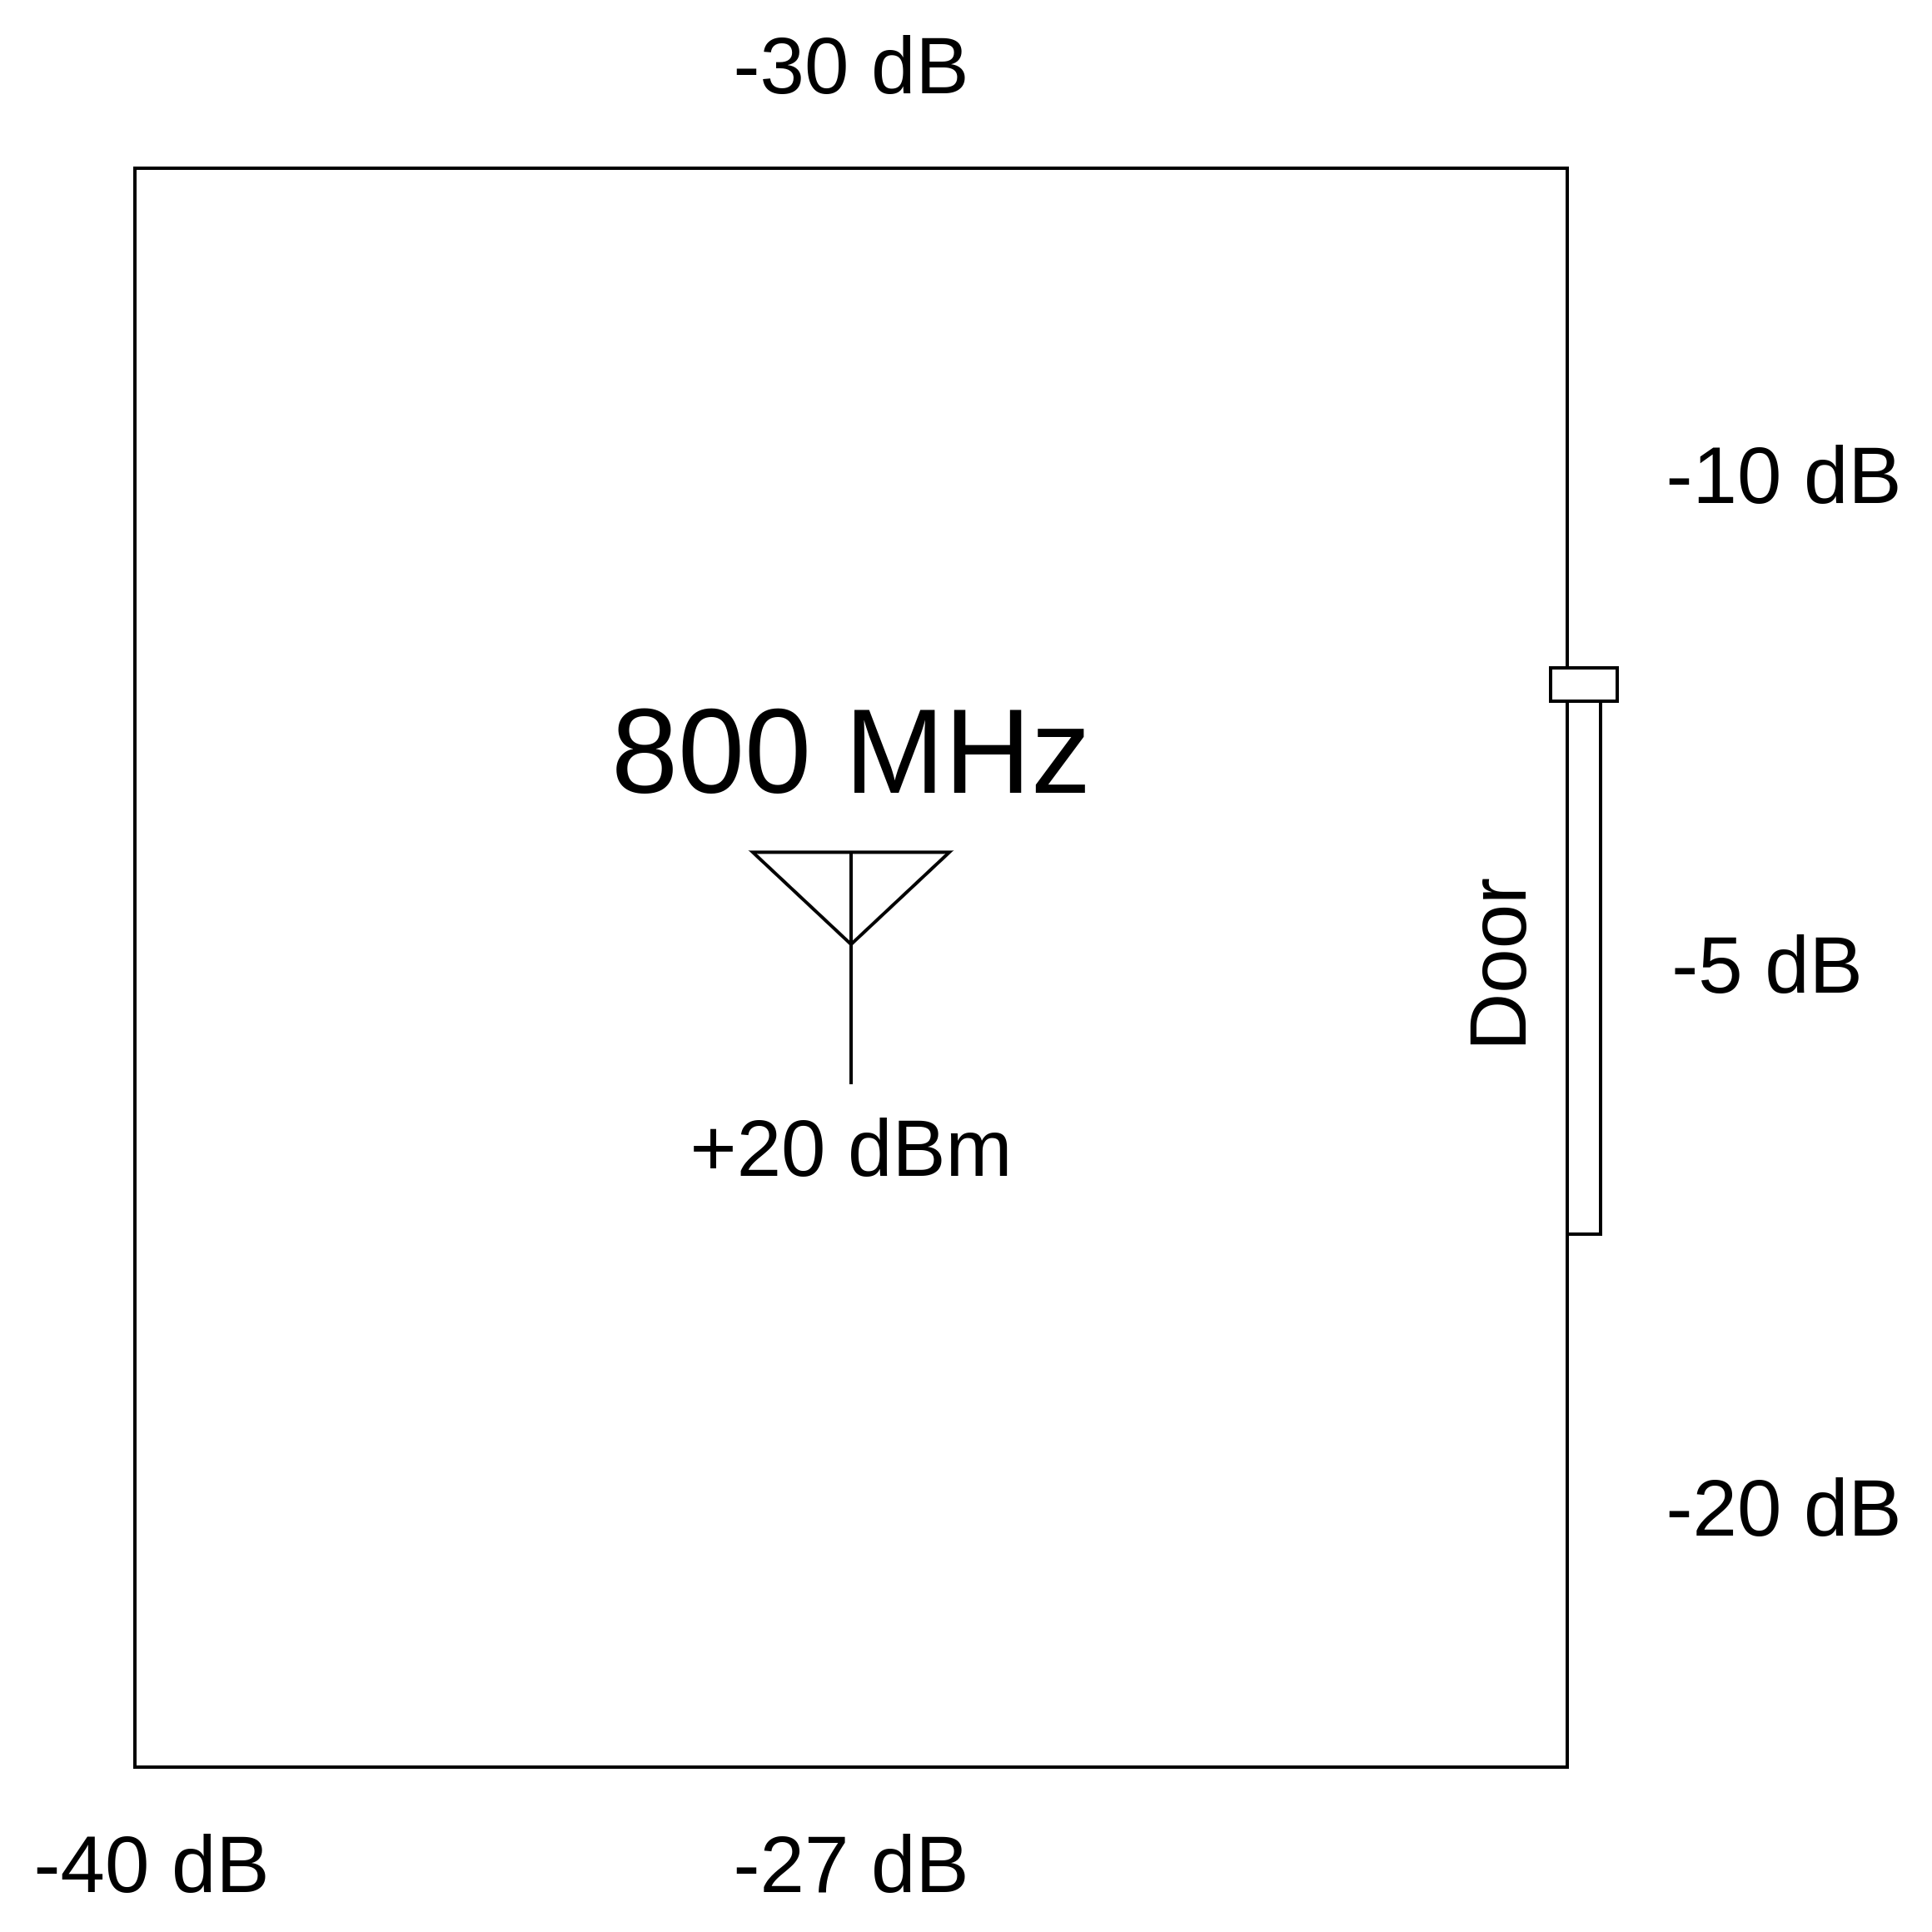
\includegraphics[width=0.85\linewidth]{images/schematics/800MHz_result.png}
\caption{Power level detected outside the screen room for a +20$\thinspace$dBm signal emitted at 800$\thinspace$MHz.}
\label{fig:800MHz_result}
\end{figure}

\begin{figure}[H]
\centering
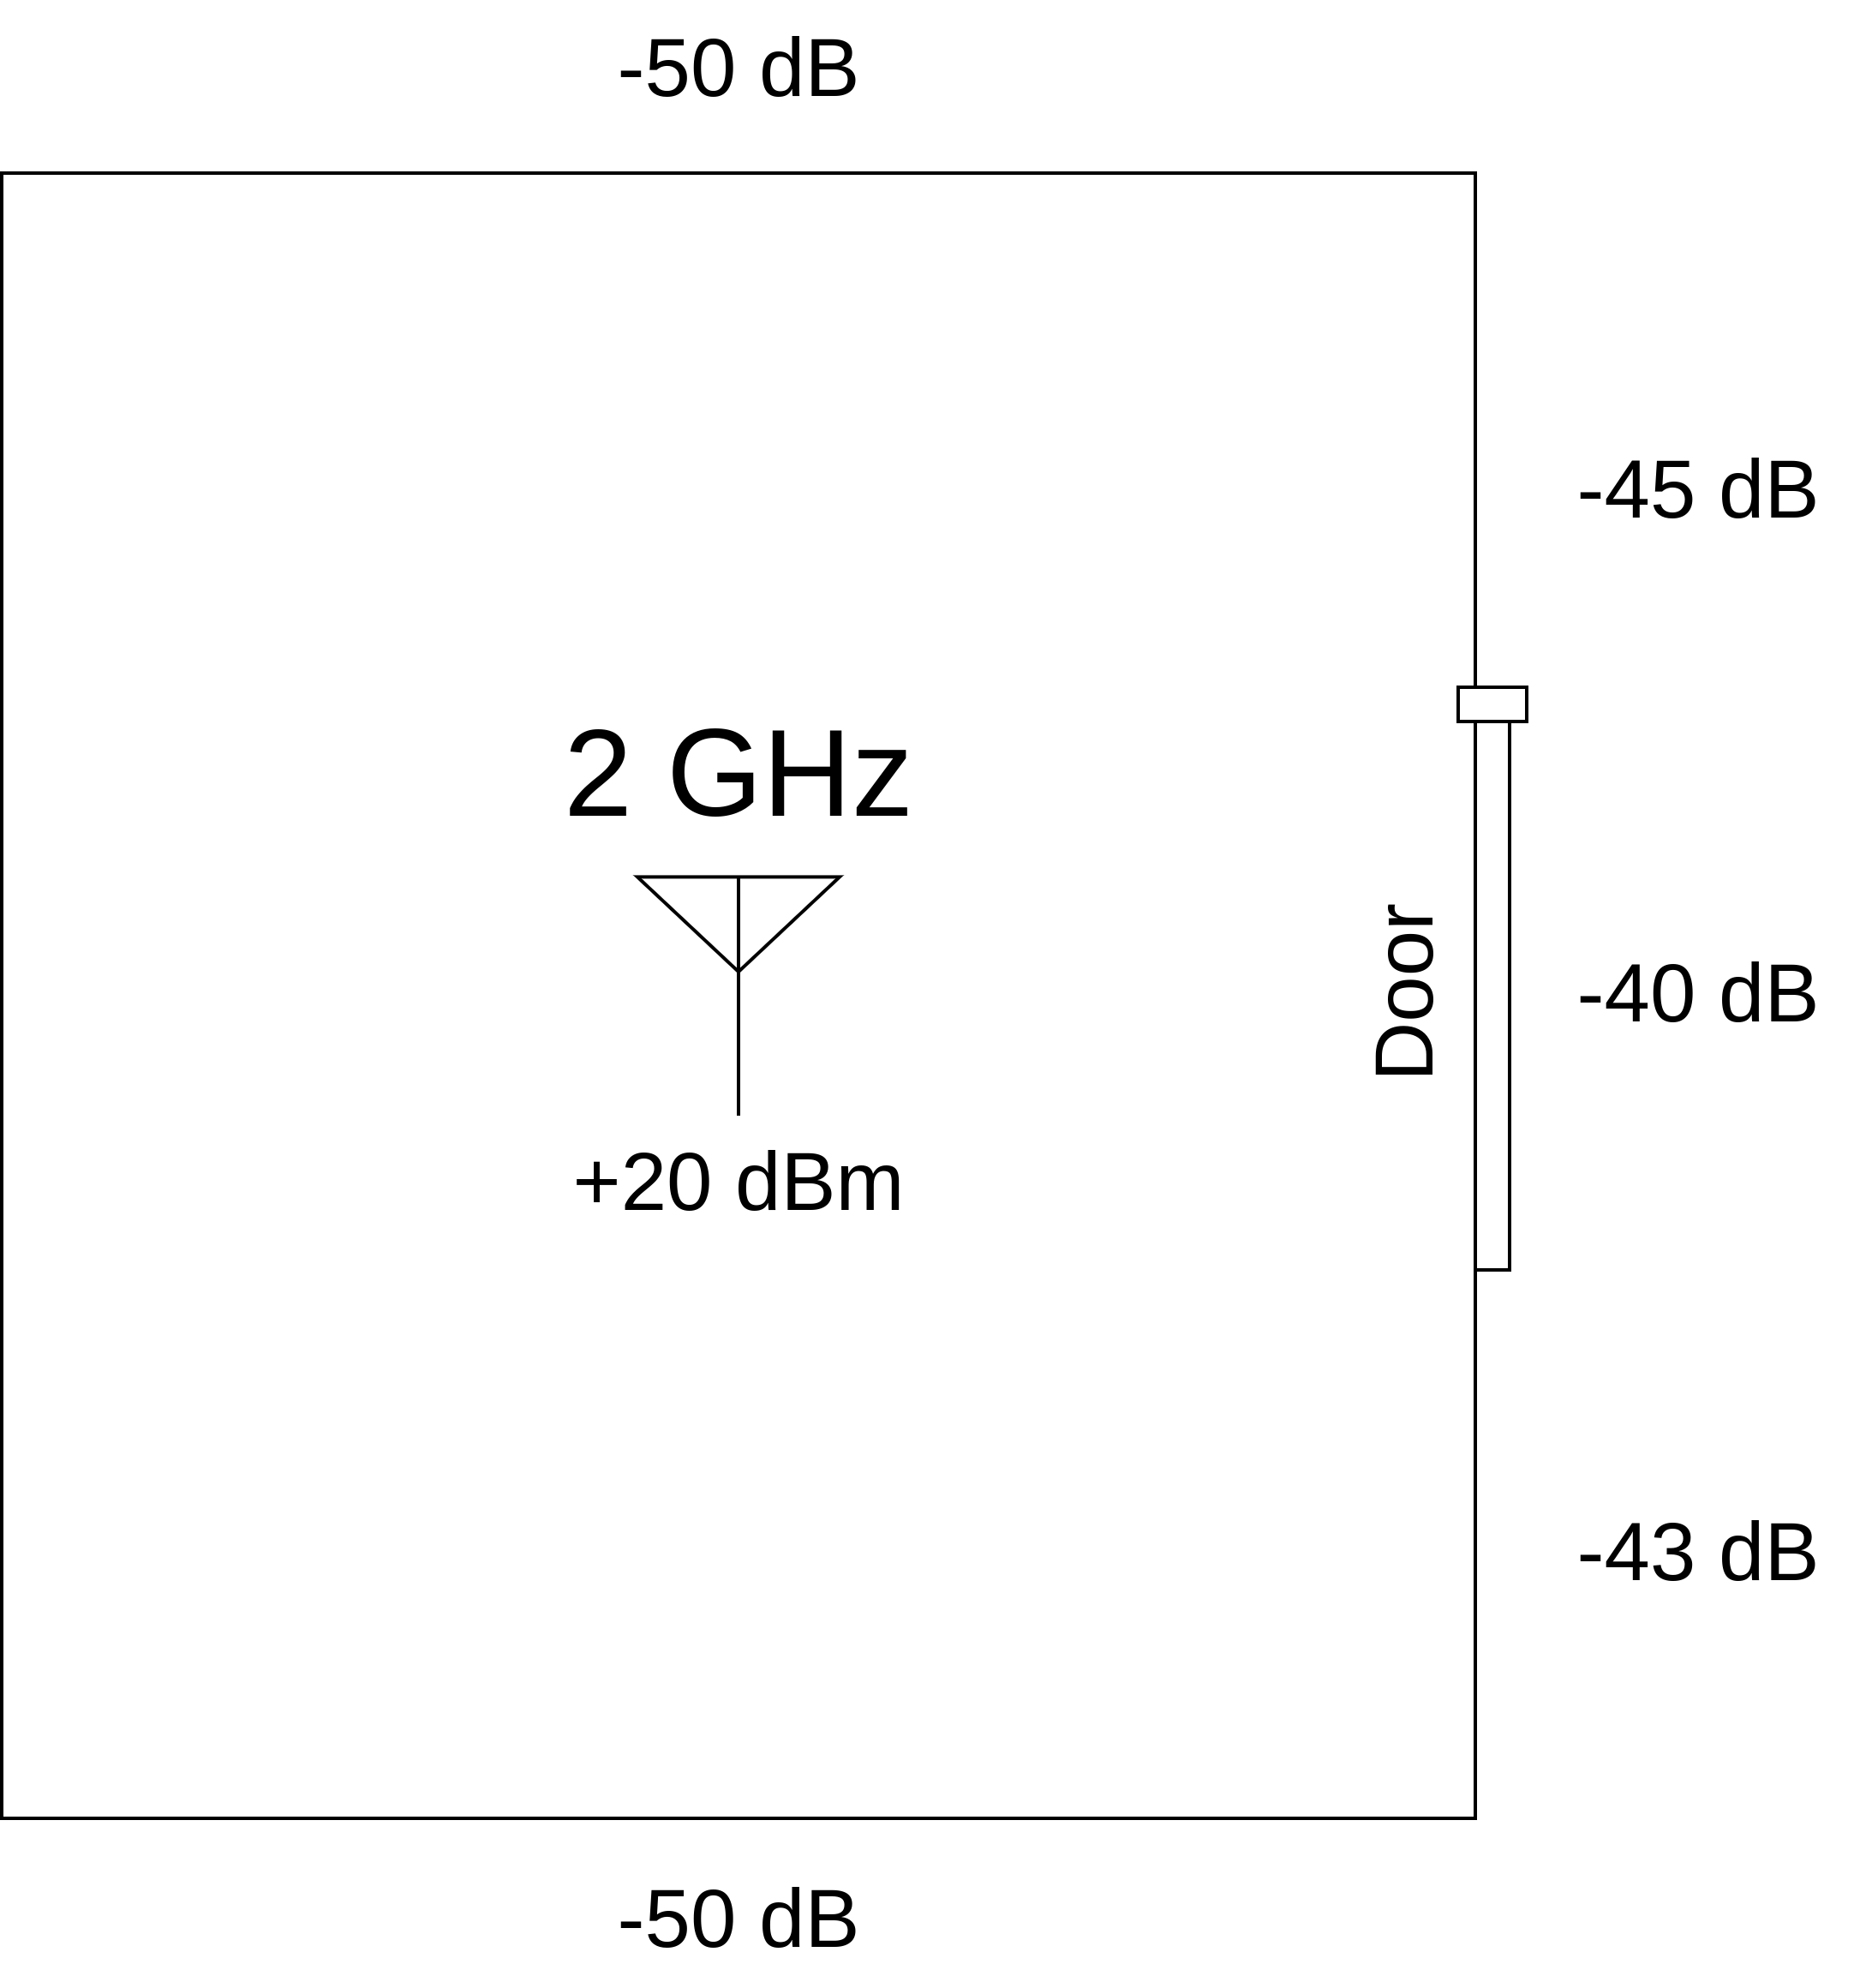
\includegraphics[width=0.85\linewidth]{images/schematics/2GHz_result.png}
\caption{Power level detected outside the screen room for a +20$\thinspace$dBm signal emitted at 2$\thinspace$GHz.}
\label{fig:2GHz_result}
\end{figure}

\appendix
% ----------------------------------------------------------------

% To include pages from other PDFs
% 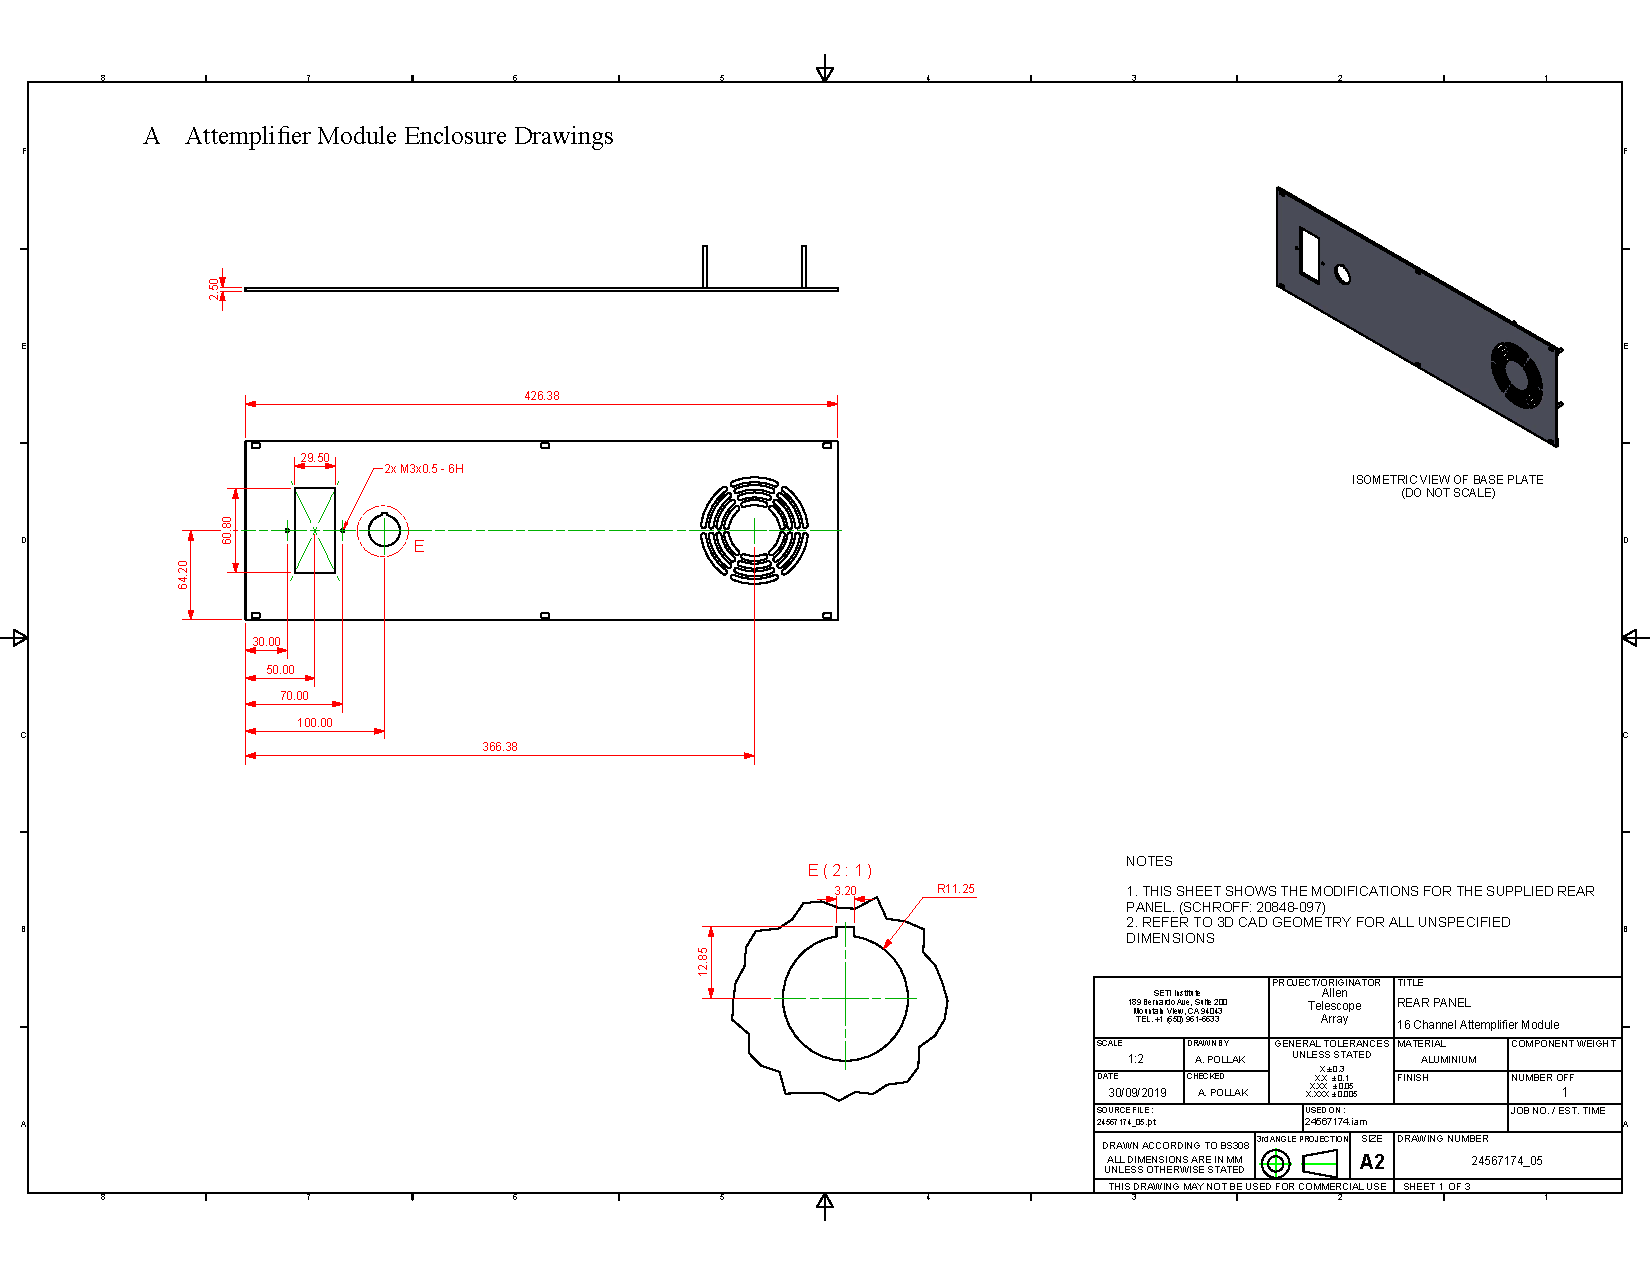
\includepdf[pages=-, landscape=true]{Documentation/PDFs/24567174_05(copy).pdf}


%----------------------------------------------------------------------------------------
%	Appendix: 
%----------------------------------------------------------------------------------------

%
%\begin{figure}[H]
%\centering
%\includegraphics[width=1\linewidth]{<path>/picture.png}
%\caption{Caption}
%\label{fig:LABEL}
%\end{figure}
%

\end{document}
